\begin{figure}[htb!] 
\centering
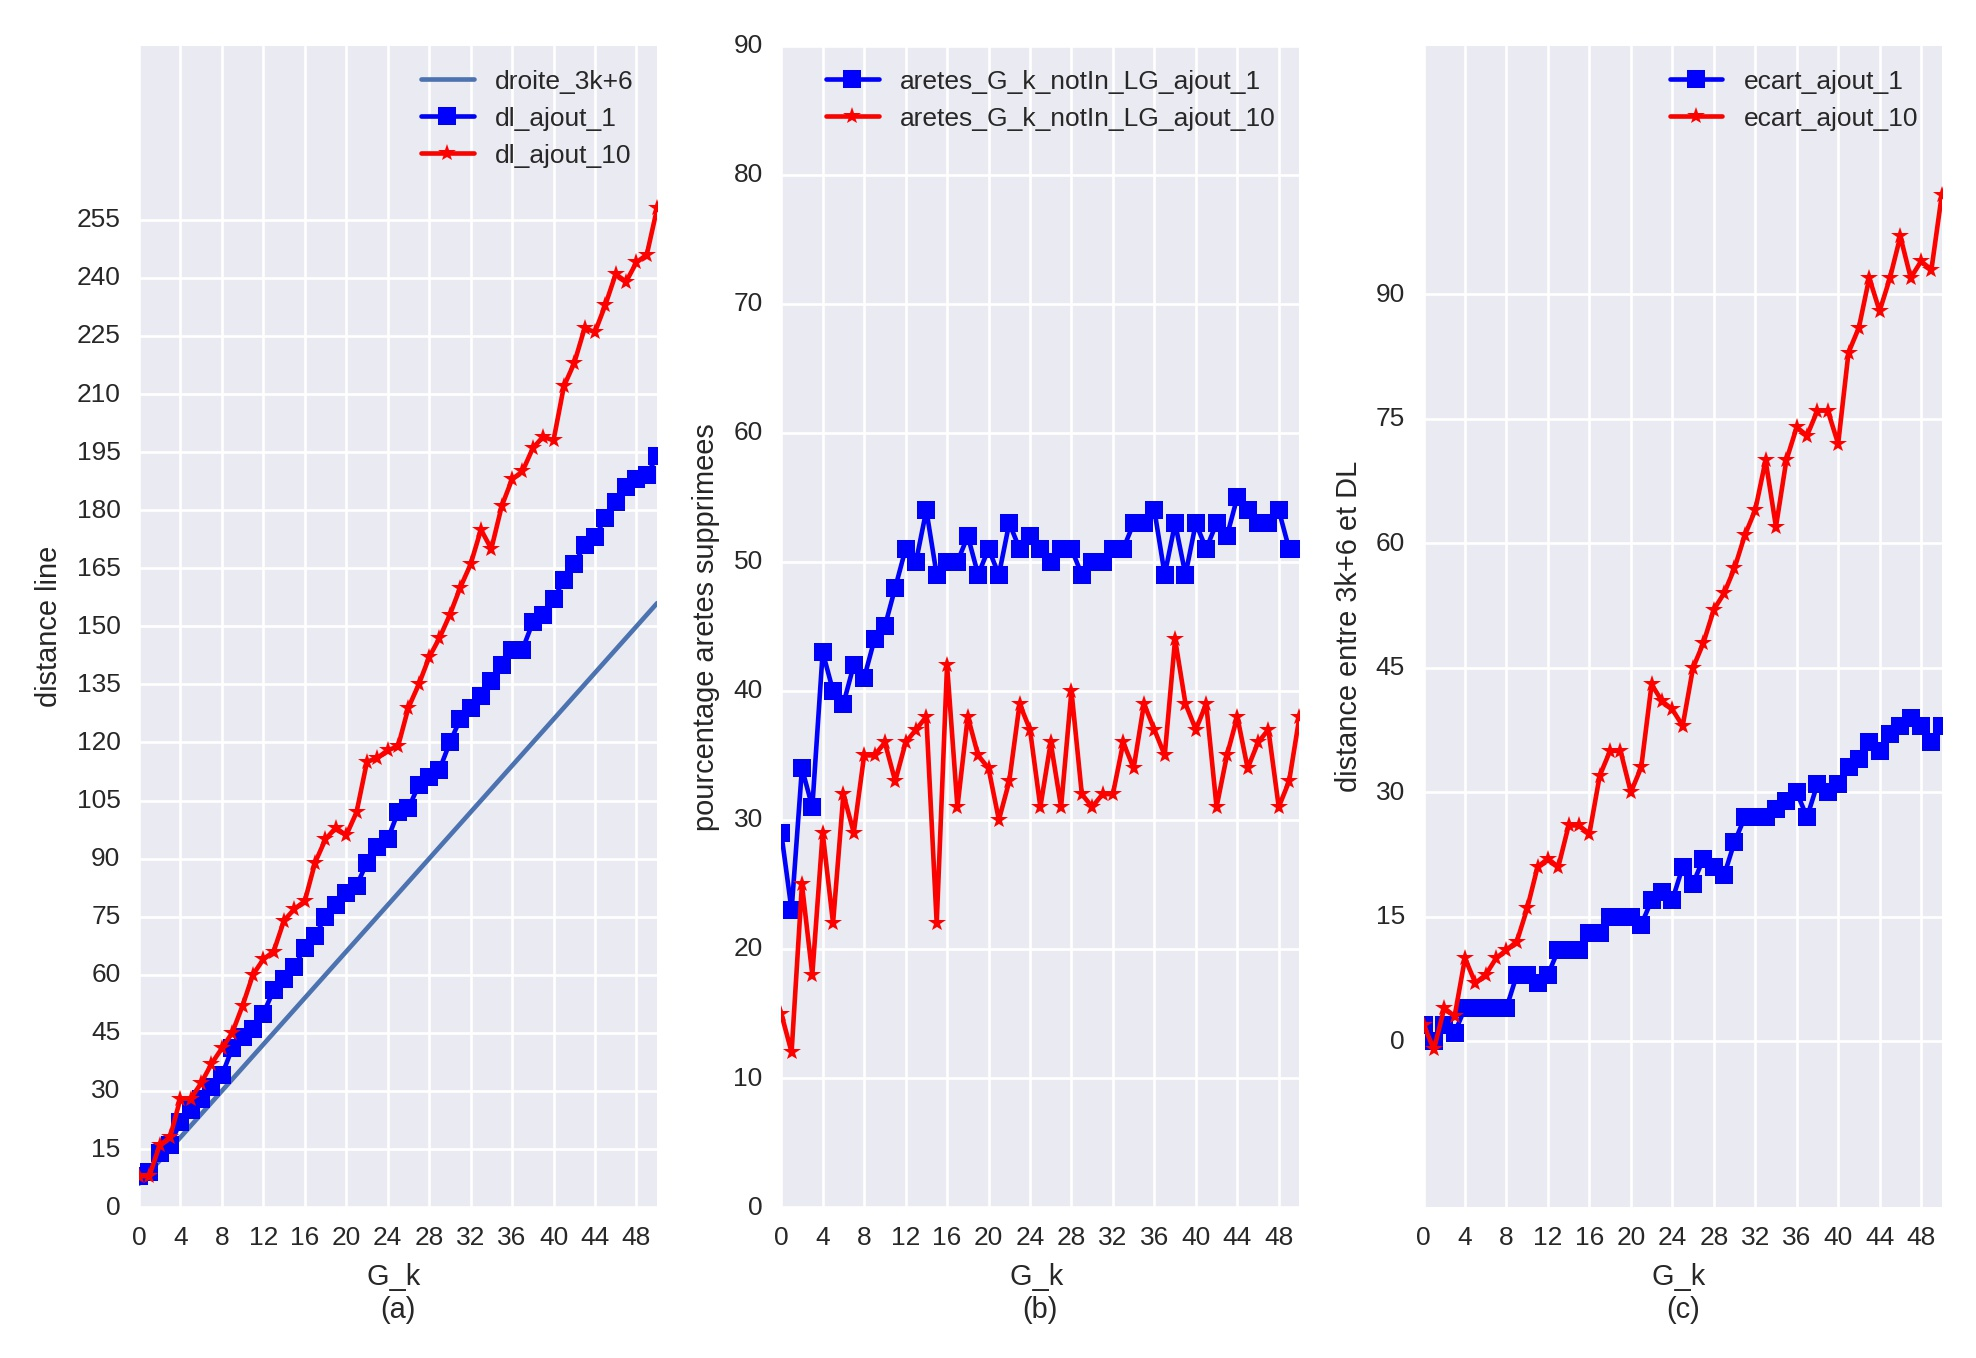
\includegraphics[scale=0.250]{comparaison_prior_ajout_wi_1_ajout_wi_10_distance_line_vs_3k_6_graphe_iourte.jpeg}
\caption{  (a) fonction de co\^ut {\em ajout} : la courbe {\em dl\_ajout\_1} d\'esigne la correction par la priorisation des ar\^etes ajout\'ees avec un poids $\phi^{+} = 1$  pour une ar\^ete ajout\'ee et un poids $\phi^{-} = 1$  pour une ar\^ete supprim\'ee.
 La courbe {\em dl\_ajout\_10} d\'esigne la correction par la priorisation des ar\^etes ajout\'ees avec un poids $\phi^{+} = 1$  pour une ar\^ete ajout\'ee et un poids $\phi^{-} = 10$  pour une ar\^ete supprim\'ee,
 (b) taux de suppression d'ar\^etes dans  $G_0^k$ pour les priorisations  {\em dl\_ajout\_1} et  {\em dl\_ajout\_10},
(c) la diff\'erence de distances line entre les priorisations {\em dl\_ajout\_1} et  {\em dl\_ajout\_10}  et la droite $y=3k+6$. }
\label{priorAjout1Ajout10} 
\end{figure}

Dans la fonction de co\^ut {\em ajout}, nous comparons deux courbes. La premi\`ere est la courbe {\em dl\_ajout\_1} qui a \'et\'e d\'ecrite pr\'ec\'edemment ($\phi^{+} = \phi^{-} = 1$ ). la seconde est la courbe {\em dl\_ajout\_10} qui d\'esigne la priorisation des ar\^etes ajout\'ees en attribuant un poids $\phi^{+} = 1$ pour l'ajout d'ar\^etes et un poids $\phi^{-} = 10$ pour la suppression d'ar\^etes.
\newline
Dans la figure \ref{priorAjout1Ajout10}(a), la courbe {\em dl\_ajout\_10} fournit des distances line sup\'erieure \`a celles de la courbe  {\em dl\_ajout\_1}. L'\'ecart de distances line {\em ecart\_ajout\_1} entre la droite $y = 3k + 6 $ et la courbe {\em dl\_ajout\_1} croit lin\'eairement alors que celui entre les courbes {\em dl\_ajout\_10} et $y = 3k + 1 $ est une succession de croissance et de d\'ecroissance (voir figure \ref{priorAjout1Ajout10}(c)). 
Cette d\'ecroissance constat\'ee \`a $k=\{6,20,26,36,42\}$ correspond \`a l'ajout de peu d'ar\^etes (extremums inf\'erieurs de la courbe {\em aretes\_G\_k\_notIn\_LG\_ajout\_10} de la figure \ref{priorAjout1Ajout10}(b)) dans les graphes $G_0^k$.
 Il se d\'eduit que la courbe {\em dl\_ajout\_10} ajoute beaucoup d'ar\^etes dans $G_0^k$ par rapport \`a la courbe  {\em dl\_ajout\_1}. 
Ce qui est normal puisque l'hypoth\`ese de depart est la priorisation de l'ajout d'ar\^etes.
De m\^eme, la croissante lin\'eaire de {\em ecart\_ajout\_1} decoule de la suppression d'ar\^etes majoritairement que nous remarquons dans la figure \ref{priorAjout1Ajout10}(b) avec la courbe {\em aretes\_G\_k\_notIn\_LG\_ajout\_1}. Les ar\^etes ajout\'ees sont peu nombreuses entrainant le rapprochement entre la courbe {\em dl\_ajout\_1} et la droite $y = 3k +6$ (voir figure \ref{priorAjout1Ajout10}(c)).
\newline
Nous concluons que l'ajout des ar\^etes au detriment de la suppression pendant la phase de correction donne de moins bons r\'esultats par rapport \`a la priorisation {\em unitaire}. La priorisation {\em ajout} ajoute majoritairement des ar\^etes qui l'\'eloigne de la r\'ef\'erence theorique de la distance line, la droite $y = 3k+6$.
% Toutefois, la suppression d'ar\^etes necessite 